\documentclass[12pt,a4paper]{article}
\usepackage{ctex}
\usepackage{listings}
\usepackage{xcolor}
\usepackage{fancyhdr}
\usepackage{graphicx}
\pagestyle{fancy}
\rhead{Mingchen Liu}
\lstset{
    %backgroundcolor=\color{red!50!green!50!blue!50},%代码块背景色为浅灰色
    rulesepcolor= \color{gray}, %代码块边框颜色
    breaklines=true,  %代码过长则换行
    numbers=left, %行号在左侧显示
    numberstyle= \small,%行号字体
    %keywordstyle= \color{red},%关键字颜色
    commentstyle=\color{gray}, %注释颜色
    frame=shadowbox%用方框框住代码块
    }

% Title
\title{《计算方法》课程实验报告}
\author{刘铭宸\\软件工程2003班\\U202010783}
\date{\today}
 
\begin{document}

\begin{titlepage}
\maketitle
\end{titlepage}

\tableofcontents

\newpage
\section{实际问题}
研究发现,学生的学习成绩
和其所在地区的人均年收入(地区收入)之间存在正相关性。
有关机构在对1998年美国加利福尼亚州的五年级学生
进行抽样调查后发现,测试成绩和地区收入的相关系数
大约为0.71,由此建立了负指数生长回归函数。
根据加利福尼亚数据集$^{[1]}$,
可以得知学生的测试成绩和地区收入的负指数模型为:
\begin{equation}
    TestScore=703.2[1-e^{-0.0552(I+34.0)}]
\end{equation}
其中TestScore表示测试成绩(分),
参数I表示地区收入(千美元)。

根据该模型,控制其他因素不变,
试问所在地区的人均年收入为多少的学生更有可能在考试中能够得到700分?
\section{问题求解}
该实际问题归结为求解非线性方程
$703.2[1-e^{-0.0552(I+34.0)}]=700$的根。
下面我们将用多种数值解法求解此非线性方程,
并对结果进行分析。
\subsection{几何法求解}
根据迭代法的要求,
令$f(I)=703.2[1-e^{-0.0552(I+34.0)}]-700$,
经过初步计算可以知道[50,90]为该方程的一个隔离区间,
故在此我们将实验区间定为[50,90],
允许误差大小定为0.0001千美元,
对二分法、弦截法和Steffensen方法进行试验,
并对三种方法进行比较分析。
\subsubsection{二分法}
首先我们可以根据预设精度用公式:
\begin{equation}
    k>\frac{ln(b-a)-ln(2\xi)}{ln2}
\end{equation}
计算出二分的最少次数,其中k为二分次数,
b和a分别为实验区间的上界和下界,
$\xi$为预设精度,
在本问题中为$10^{-4}$。

可得满足精度要求的最少二分次数为18次。
根据课本2.1节关于二分法的介绍,编写代码如下:
\begin{lstlisting}[language={java}]
    public class Dichotomy {
        public static double f(double I){
            return 703.2*(1-Math.exp(-0.0552*(I+34.0)))-700;
        }
    
        public static void main(String[] args) {
            double a = 50, b = 90;
            while(b-a >= 0.0001){
                double c = (a+b)/2;
                if(f(c)==0)
                    break;
                else if(f(a)*f(c)<0)
                    b = c;
                else
                    a = c;
                System.out.println(b-a);
            }
            System.out.println("I = "+(a+b)/2);
        }
    }
\end{lstlisting}
~\\
计算结果如下表:
\begin{table}[ht]
    \centering
    \begin{tabular}{|c|c|c|c|c|c|} 
     \hline
     迭代次数 & 1 & 2 & 3 & 4 & 5 \\ [0.5ex] 
     \hline
     误差 & 20.000000 & 10.000000 & 5.000000 & 2.500000 & 1.250000 \\ 
     \hline
     迭代次数 & 6 & 7 & 8 & 9 & 10 \\
     \hline
     误差 & 0.625000 & 0.312500 & 0.156250 & 0.078125 & 0.039063 \\
     \hline
     迭代次数 & 11 & 12 & 13 & 14 & 15 \\
     \hline
     误差 & 0.019531 & 0.009766 & 0.004883 & 0.002441 & 0.001221 \\
     \hline
     迭代次数 & 16 & 17 & 18 & 19 & \\
     \hline
     误差 & 0.000610 & 0.000305 & 0.000153 & 0.000076 & \\
     \hline
     I & \multicolumn{5}{c|}{63.690071} \\
     \hline
    \end{tabular}
    \caption{二分法的计算结果}
    \label{table:1}
\end{table}
    ~\\~\\~\\~\\~\\~\\~\\
    结果分析:

    结果显示,二分法总共迭代了19次,
    最终求得I=63.690071,
    即所在地区的人均年收入达到约63690美元时,
    学生更有可能获得700分。
    最终迭代误差为7.62939453125e-5,
    显然达到了实验预设误差要求。

\subsubsection{弦截法}
弦截法的一般迭代表达式为:
\begin{equation}
    x_{k+1}=x_k-\frac{x_k-x_{k-1}}{f(x_k)-f(x_{k-1})}f(x_k),~~~~k=1,2,\dots
\end{equation}
在本问题中,取初始迭代值$x_0=50, x_1=90$

根据课本2.2节关于弦截法的介绍,编写代码如下:
\begin{lstlisting}[language={java}]
    public class Secant {
        public static double f(double I){
            return 703.2*(1-Math.exp(-0.0552*(I+34.0)))-700;
        }

        public static void main(String[] args) {
            double x0 = 50, x1 = 90;
            double x2 = x1-(x1-x0)*f(x1)/(f(x1)-f(x0));
            double tol = 0.0001;
            while(Math.abs(x2-x1)>=tol){
                x0 = x1;
                x1 = x2;
                x2 = x1-(x1-x0)*f(x1)/(f(x1)-f(x0));
                System.out.println(Math.abs(x2-x1));
            }
            System.out.println("I = "+x2);
        }
    }
\end{lstlisting}
~\\
计算结果如下表:
\begin{table}[ht]
    \centering
    \begin{tabular}{|c|c|c|c|c|} 
     \hline
     迭代次数 & 1 & 2 & 3 & 4 \\ [0.5ex] 
     \hline
     误差 & 20.551021 & 13.239997 & 2.079753 & 0.812050 \\ 
     \hline
     迭代次数 & 5 & 6 & 7 & \\
     \hline
     误差 & 0.061945 & 0.001264 & 0.000002 & \\
     \hline
     I & \multicolumn{4}{c|}{63.690046} \\
     \hline
    \end{tabular}
    \caption{弦截法的计算结果}
    \label{table:2}
\end{table}
~\\
结果分析:

结果显示,弦截法总共迭代了7次,
最终求得I=63.690046,
即所在地区的人均年收入达到约63690美元时,
学生更有可能获得700分。
最终迭代误差为2.119659875177149e-6,
显然达到了实验预设误差要求。

\subsubsection{Steffensen方法}
Steffensen方法的一般迭代表达式为:
\begin{equation}
    x_{k+1}=x_k-\frac{f^2(x_k)}{f(x_k)-f(x_k-f(x_k))},~~~~k=1,2,\dots
\end{equation}
在本问题中,取初始迭代值$x_0=50$

根据课本2.2节关于Steffensen方法的介绍,编写代码如下:
\begin{lstlisting}[language={java}]
    public class Steffensen {
        public static double f(double I){
            return 703.2*(1-Math.exp(-0.0552*(I+34.0)))-700;
        }
    
        public static void main(String[] args) {
            double x0 = 50;
            double x1 = x0-f(x0)*f(x0)/(f(x0)-f(x0-f(x0)));
            while(Math.abs(x1-x0)>=0.0001){
                x0 = x1;
                x1 = x0-f(x0)*f(x0)/(f(x0)-f(x0-f(x0)));
                System.out.println(Math.abs(x1-x0));
            }
            System.out.println("I = "+x1);
        }
    }
\end{lstlisting}
~\\
计算结果如下表:
\begin{table}[ht]
    \centering
    \begin{tabular}{|c|c|c|} 
     \hline
     迭代次数 & 1 & 2 \\ [0.5ex] 
     \hline
     误差 & 2.890429 & 0.201702 \\ 
     \hline
     迭代次数 & 3 & 4 \\
     \hline
     误差 & 0.000929 & 1.960079e-8 \\
     \hline
     I & \multicolumn{2}{c|}{63.690046} \\
     \hline
    \end{tabular}
    \caption{弦截法的计算结果}
    \label{table:3}
\end{table}
~\\~\\~\\~\\
结果分析:

结果显示,Steffensen方法总共迭代了4次,
最终求得I=63.690046,
即所在地区的人均年收入达到约63690美元时,
学生更有可能获得700分。
最终迭代误差为1.9600790324147965e-8,
显然达到了实验预设误差要求。

\subsubsection{比较分析}
将三种方法每次迭代产生的误差大小绘制得到如图1所示。
从图中可以看到,三种方法最终的误差均趋于零,
即我们可以认为三种方法都是收敛的。
另外,初值取50时的Steffensen方法收敛速度最快,
仅用4次就达到了预设精度要求;
弦截法次之,二分法最慢,
分别用了7次和19次迭代才达到预设精度要求。
但是,作为一种单步法,
Steffensen方法的收敛速度和初值的选取有很大关系。
当将初值$x_0$取为98时,得到的结果如图二所示。
可以看到,此时Steffensen方法的收敛速度与效果低于弦截法。
实验中得到的结果也是符合课本上的理论分析的。
\begin{figure}
    \centering
    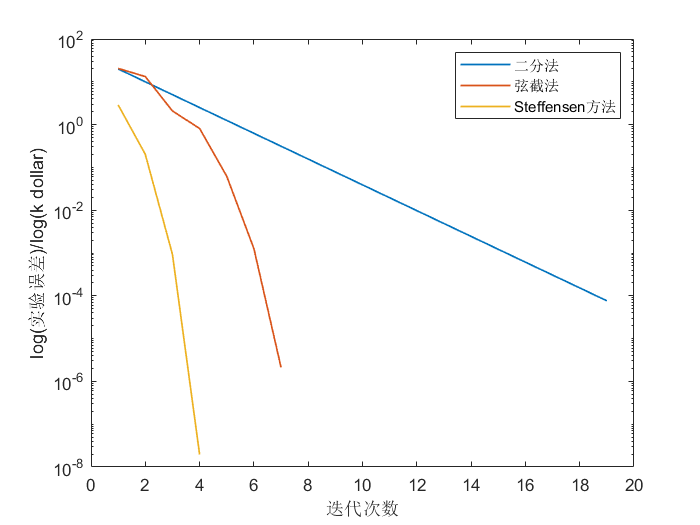
\includegraphics[scale=0.6]{pic01.png}
    \caption{几何法的实验误差与迭代次数对比}
    \label{fig:1}
\end{figure}
\begin{figure}
    \centering
    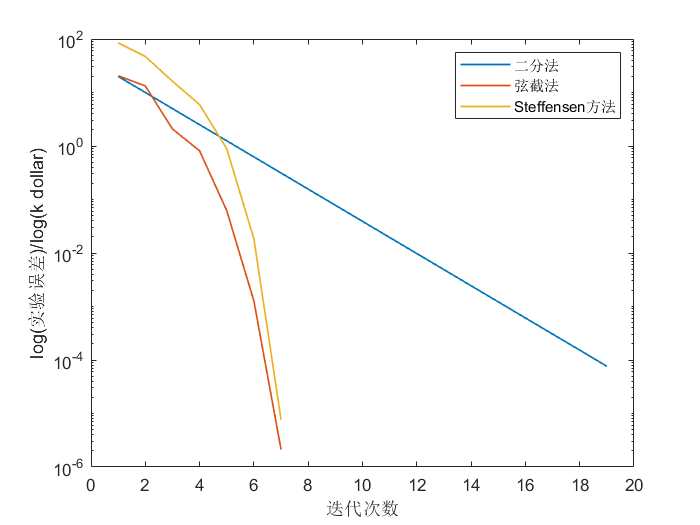
\includegraphics[scale=0.6]{pic02.png}
    \caption{初值取98时的Steffensen方法与二分法、弦截法的对比}
    \label{fig:2}
\end{figure}
\subsection{迭代法求解}
根据迭代法的要求,可将原方程等价写为
$I=703.2[1-e^{-0.0552(I+34.0)}]-700+I$的形式。
下面我们将用多种数值解法求解此非线性方程,并对结果进行分析。
\subsubsection{Picard迭代法}
构造Picard迭代法的迭代格式:
\begin{equation}
    I_{k+1}=703.2[1-e^{-0.0552(I_k+34.0)}]-700+I_k,~~~k=0,1,2,\dots
\end{equation}

首先我们可以根据课本2.3节介绍的Picard迭代法的局部收敛性判据对其敛散性进行分析:

(1)对迭代函数$\phi(I)$求导得$\phi^{'}(I)=38.81664e^{-0.0552(I+34.0)}+1$,
可知导函数在任意区间内都连续可微。

(2)对于任意I,都有$|\phi^{'}(I)|>1$成立。

所以该迭代格式不满足局部收敛性判据,
同理可以得到此格式亦不满足全局收敛性判据。
但由于此二者皆为迭代格式收敛的充分不必要条件,
我们仍无法确定其发散。

下面通过编程进行分析。编写代码如下:
\begin{lstlisting}[language={java}]
    public class Picard {
        public static double fai(double I){
            return 703.2*(1-Math.exp(-0.0552*(I+34.0)))-700+I;
        }
    
        public static void main(String[] args) {
            double x0 = 50;
            double x1 = fai(x0);
            while(Math.abs(x1-x0)>=0.0001){
                System.out.println(Math.abs(x1-x0));
                x0 = x1;
                x1 = fai(x0);
            }
            System.out.println(Math.abs(x1-x0));
            System.out.println("I = "+x1);
        }
    }
\end{lstlisting}

计算结果如下表:
\begin{table}[ht]
    \centering
    \begin{tabular}{|c|c|c|c|c|c|} 
     \hline
     迭代次数 & 1 & 2 & 3 & 4 & 5 \\ [0.5ex] 
     \hline
     误差 & 3.613060 & 5.116839 & 7.831246 & 13.796654 & 33.200840 \\ 
     \hline
     迭代次数 & 6 & 7 & 8 & 9 & \\
     \hline
     误差 & 224.329122 & 54311455 & Infinity & NaN & \\
     \hline
     I & \multicolumn{5}{c|}{-Infinity} \\
     \hline
    \end{tabular}
    \caption{Picard迭代法的计算结果}
    \label{table:4}
\end{table}
~\\
结果分析:

可以看到实验误差趋向于无穷,
可知该迭代格式是发散的,
对其使用Picard迭代法无法求出正确结果。

\subsubsection{Aitken加速迭代法(含导数)}
含导数的Aitken加速迭代格式为:
\begin{equation}
    x_{k+1}=(1-l)^{-1}[\phi(x_k)-lx_k],~~~k=0,1,\dots
\end{equation}
其中$l=\phi^{'}(x^{*})\approx\phi^{'}(\frac{50+90}{2})=\phi^{'}(70)$,
初始迭代值$x_0=50$

根据课本2.4节关于Aitken加速迭代法的介绍,编写代码如下:
\begin{lstlisting}[language={java}]
    public class Aitken_derivative {
        public static double fai(double I){
            return 703.2*(1-Math.exp(-0.0552*(I+34.0)))-700+I;
        }
    
        public static double dfai(double I){
            return 38.81664*Math.exp(-0.0552*(I+34.0))+1;
        }
    
        public static void main(String[] args) {
            double l = dfai((50+90)/2.0);
            double x0 = 50;
            double x1 = (fai(x0)-l*x0)/(1-l);
            while(Math.abs(x1-x0)>=0.0001){
                System.out.println(Math.abs(x1-x0));
                x0 = x1;
                x1 = (fai(x0)-l*x0)/(1-l);
            }
            System.out.println(Math.abs(x1-x0));
            System.out.println("I = "+x1);
        }
    }
\end{lstlisting}

计算结果如下表:
\begin{table}[ht]
    \centering
    \begin{tabular}{|c|c|c|c|c|c|} 
     \hline
     迭代次数 & 1 & 2 & 3 & 4 & 5 \\ [0.5ex] 
     \hline
     误差 & 28.977104 & 14.627290 & 0.917859 & 0.368246 & 0.155581 \\ 
     \hline
     迭代次数 & 6 & 7 & 8 & 9 & 10 \\
     \hline
     误差 & 0.064433 & 0.026914 & 0.011203 & 0.004670 & 0.001945 \\
     \hline
     迭代次数 & 11 & 12 & 13 & 14 &  \\
     \hline
     误差 & 0.000811 & 0.000338 & 0.000141 & 0.000059 & \\
     \hline
     I & \multicolumn{5}{c|}{63.690063} \\
     \hline
    \end{tabular}
    \caption{含导数的Aitken加速迭代法的计算结果}
    \label{table:5}
\end{table}
~\\
结果分析:

结果显示,不含导数的Aitken加速迭代法总共迭代了14次,
最终求得I=63.690063,
即所在地区的人均年收入达到约63690美元时,
学生更有可能获得700分。
最终迭代误差为5.864194860549787e-5,
显然达到了实验预设误差要求。

\subsubsection{Aitken加速迭代法(不含导数)}
不含导数的Aitken加速迭代格式为:
\begin{equation}
    \left\{
\begin{array}{c}
	\tilde{x}_{k+1}=\phi(x_k),~~\hat{x}_{k+1}=\phi(\tilde{x}_{k+1})\\
	x_{k+1}=\hat{x}_{k+1}-\frac{(\hat{x}_{k+1}-\tilde{x}_{k+1})^2}{\hat{x}_{k+1}-2\tilde{x}_{k+1}+x_k}
\end{array}
\right. 
\end{equation}
取初始迭代值$x_0=50$

根据课本2.4节关于Aitken加速迭代法的介绍,编写代码如下:
\begin{lstlisting}[language={java}]
    public class Aitken_noderivative {
        public static double fai(double I){
            return 703.2*(1-Math.exp(-0.0552*(I+34.0)))-700+I;
        }
    
        public static void main(String[] args) {
            double x0 = 50;
            double x1 = fai(x0);
            double x2 = fai(x1);
            double x3 = x2-(x2-x1)*(x2-x1)/(x2-2*x1+x0);
            while(Math.abs(x3-x0)>=0.0001){
                System.out.println(Math.abs(x3-x0));
                x0 = x3;
                x1 = fai(x0);
                x2 = fai(x1);
                x3 = x2-(x2-x1)*(x2-x1)/(x2-2*x1+x0);
            }
            System.out.println(Math.abs(x3-x0));
            System.out.println("I = "+x3);
        }
    }    
\end{lstlisting}
~\\
计算结果如下表:
\begin{table}[ht]
    \centering
    \begin{tabular}{|c|c|c|c|} 
     \hline
     迭代次数 & 1 & 2 & 3 \\ [0.5ex] 
     \hline
     误差 & 8.680931 & 4.254293 & 0.736539 \\ 
     \hline
     迭代次数 & 4 & 5 & \\
     \hline
     误差 & 0.018273 & 0.000011 & \\
     \hline
     I & \multicolumn{3}{c|}{63.690046} \\
     \hline
    \end{tabular}
    \caption{不含导数的Aitken加速迭代法的计算结果}
    \label{table:6}
\end{table}
~\\
结果分析:

结果显示,不含导数的Aitken加速迭代法总共迭代了5次,
最终求得I=63.690046,
即所在地区的人均年收入达到约63690美元时,
学生更有可能获得700分。
最终迭代误差为1.0853231756868809e-5,
显然达到了实验预设误差要求。

\subsubsection{Newton迭代法}
Newton迭代法的一般表达式为:
\begin{equation}
    x_k=x_{k-1}-\frac{f(x_k)}{f^{'}(x_k)},~~~k=1,2,\dots
\end{equation}
取初始迭代值$x_0=50$

根据课本2.5节关于Newton迭代法的介绍,编写代码如下:
\begin{lstlisting}[language={java}]
    public class Newton {
        public static double f(double I){
            return 703.2*(1-Math.exp(-0.0552*(I+34.0)))-700;
        }
    
        public static double df(double I){
            return 38.81664*Math.exp(-0.0552*(I+34.0));
        }
    
        public static void main(String[] args) {
            double x0 = 50;
            double x1 = x0-f(x0)/df(x0);
            while(Math.abs(x1-x0)>=0.0001){
                System.out.println(Math.abs(x1-x0));
                x0 = x1;
                x1 = x0-f(x0)/df(x0);
            }
            System.out.println(Math.abs(x1-x0));
            System.out.println("I = "+x1);
        }
    } 
\end{lstlisting}
~\\
计算结果如下表:
\begin{table}[ht]
    \centering
    \begin{tabular}{|c|c|c|c|} 
     \hline
     迭代次数 & 1 & 2 & 3 \\ [0.5ex] 
     \hline
     误差 & 9.607135 & 3.655517 & 0.422392 \\ 
     \hline
     迭代次数 & 4 & 5 & \\
     \hline
     误差 & 0.005001 & 0.0000007 & \\
     \hline
     I & \multicolumn{3}{c|}{63.690046} \\
     \hline
    \end{tabular}
    \caption{Newton迭代法的计算结果}
    \label{table:7}
\end{table}
~\\
结果分析:

结果显示,Newton迭代法总共迭代了5次,
最终求得I=63.690046,
即所在地区的人均年收入达到约63690美元时,
学生更有可能获得700分。
最终迭代误差为6.905348826080626e-7,
显然达到了实验预设误差要求。

\subsubsection{比较分析}
将四种方法每次迭代产生的误差大小绘制得到如图3所示。
从图中可以看到,Aitken加速迭代法和Newton迭代法最终的误差均趋于零,
即我们可以认为这三种方法都是收敛的;
而Picard迭代法最终趋向于无穷,对于本问题中构造的迭代格式是发散的。
根据课本2.7节关于迭代法的收敛阶的介绍,我们可以计算出这三种方法的收敛阶。
对于含导数的Aitken加速迭代法,其迭代函数为$(1-l)^{-1}[\phi(x_k)-lx_k]$,
记为$\Phi(x)$,可得:
$$
\Phi^{'}(x^{*})=(1-l)^{-1}[\phi^{'}(x^{*})-l]=0
$$
$$
\Phi^{''}(x^{*})=(1-l)^{-1}\Phi^{''}(x^{*})=-38.81664*0.0552e^{-0.0552(x^{*}+34)}<0
$$

由于$\Phi(x)$在$x^{*}$处连续可微,
可以得出含导数的Aitken加速迭代法是线性收敛的;
同时也可证明在本问题的迭代格式下,
含导数的Aitken加速迭代法是平方收敛的;
又因为$f^{'}(x^{*})\neq0$,所以$x^{*}$是单根,故Newton迭代法也是平方收敛的。
这也与实验得到的结果相符合。从图中可以看到,含导数的Aitken加速迭代法收敛速度最慢,
而Newton迭代法要比不含导数的Aitken加速迭代法收敛速度略快。
\begin{figure}
    \centering
    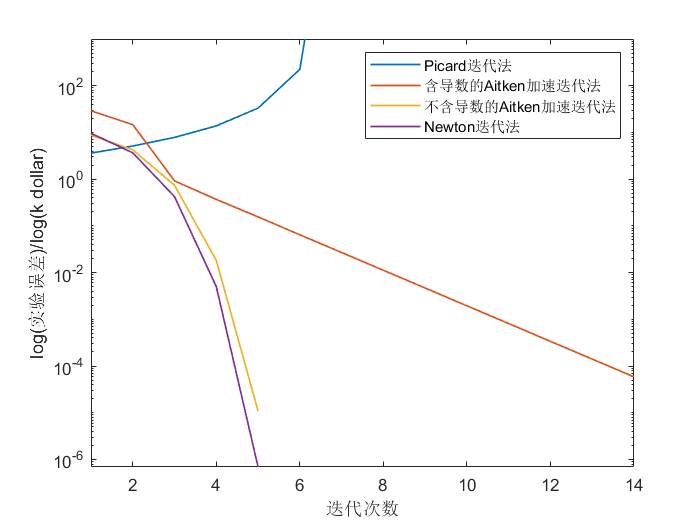
\includegraphics[scale=0.6]{pic03.png}
    \caption{迭代法的实验误差与迭代次数对比}
    \label{fig:3}
\end{figure}

\section{实验结论}
上述实验结果表明,当学生所在地区的人均年收入达到约63690美元时,
学生更有可能在测试中获得700分。

本实验在研究中存在一定的局限性。首先,学生所在地区的人均年收入并不是影响学生考试成绩的唯一原因,
其他诸如学生的学习态度、学习能力等是更显著的影响因素。
在本问题中为了研究这两者的回归模型对其它因素进行了控制,
将无法避免的影响放进了误差项之中,这样可能会引起遗漏变量偏差,
造成回归模型的不准确;
其次,被放进误差项当中的一些影响因素和本实验所研究的因变量存在相关性,
例如学生所在地区的收入在一定程度上影响着学校的教育水平和教师的授课水平,
这种相关性会引发内生性的问题,影响回归模型的一致性和有效性。
所以我认为应建立多变量的回归模型,
在控制其他变量不变的情况下再用非线性方程的数值解法对其进行分析预测,
这样得到的结果会更符合实际情况。

\section{致谢}
感谢覃婷婷老师的教学!在大学的课程学习中很少能碰见对学生如此认真负责并且
授课清楚明了的老师。在计算方法这门课上,老师更注重于教授学生公式、定理的来源与推导的思维过程,
从解决问题的角度出发向学生们介绍前人是如何一步步将这些算法构造出来的,
让我感受到数学家们也不是一下子就明白,他们也是有一个从无到有的思维过程。
在以后,那些公式定理会被我逐渐忘记,但一些解决问题的思维方式却会一直根种在脑海。
另外还要感谢老师与助教对作业的认真批改!
我在大学中从未见到对学生作业每一道题每一处细微的错误都能详细批改的老师;
每周的作业反馈也让我们及时了解自己哪里掌握的还比较薄弱,方便学生进行查缺补漏。
最后,希望覃老师的课能越办越好!

\section{参考资料}
[1]加利福尼亚数据集

https://wps.pearsoned.com/aw$\_$stock$\_$ie$\_$3/178/45691/11696965.cw/\\
index.html

[2]张诚坚,何南忠,覃婷婷.计算方法(第二版)[M].北京:高等教育出版社,2021.

[3](美)斯托克(Stock.J.H),(美)沃森(Waston,M.W.)著.沈根祥,孙燕译.计量经济学(第三版).上海:格致出版社:上海人民出版社,2012.
\end{document} 